\documentclass[12pt,a4paper]{exam}
\usepackage[utf8]{inputenc}
\usepackage[catalan]{babel}
\usepackage{graphicx}
\usepackage{geometry}
\usepackage{fancyhdr}
\usepackage{tabularx}
\usepackage{lastpage}
\usepackage{amsmath}
\usepackage{amsfonts}

% 1. MARGES I CAPÇALERA
\geometry{top=4cm, bottom=3.5cm, left=2cm, right=2cm, headheight=2.5cm}

\pagestyle{fancy}
\fancyhf{}
\fancyhead[L]{
\includegraphics[height=1.8cm]{Logo_Departament.png}} 
\fancyhead[R]{
\includegraphics[height=1.8cm]{Logo_Institut.png}}
\renewcommand{\headrulewidth}{0.4pt}

% 2. PEU DE PÀGINA
\fancyfoot[C]{
    \begin{tabularx}{\textwidth}{|>{\centering\arraybackslash}X|>{\centering\arraybackslash}X|>{\centering\arraybackslash}X|}
        \hline
        Institut Nou de Vic & Prova d'avaluació: Funcions & Pàgina \thepage\ de \pageref{LastPage} \\ \hline
    \end{tabularx}
}

\begin{document}

% 3. TAULA DE DADES
\noindent
\begingroup
\renewcommand{\arraystretch}{2}
\begin{tabularx}{\textwidth}{|X|X|c|}
    \hline
    \multicolumn{2}{|l|}{Cognoms i Nom:} & Qualificació \\ \hline
    Data: & Curs: 1r Batxillerat CCSS &  \\ \cline{1-2}
    Matèria: Matemàtiques aplicades & Prova: Examen de Funcions & \smash{\lower.5\arraystretch\hbox{}} \\ \hline
\end{tabularx}
\endgroup

\vspace{0.6cm}

\begin{questions}

% EXERCICI 1
\question (1 punt) Troba el domini de les següents funcions:
\begin{parts}
    \part $f(x) = x^2 - 5x + 6$
    \part $g(x) = \dfrac{x + 1}{x^2 - 4}$
    \part $h(x) = \sqrt{x - 5}$
    \part $i(x) = \sqrt[3]{x-4}$
\end{parts}

% EXERCICI 2
\question (1 punt) Donades les funcions $f(x) = 2x + 3$ i $g(x) = x^2 + 4$, calcula l'expressió algebraica i indica el domini de:
\begin{parts}
    \part $(f - g)(x)$
    \part $(f \cdot g)(x)$
    \part $\left(\dfrac{f}{g}\right)(x)$ 
    \part $(g \circ f)(x)$ 
\end{parts}


% EXERCICI 3
\question (1 punt) Donada la funció $f(x) = \dfrac{4}{x + 1}$:
\begin{parts}
    \part Troba la seva funció inversa $f^{-1}(x)$.
    \part Indica quin és el recorregut de la funció original $f(x)$.
\end{parts}


% EXERCICI 4
\question (1 punt) Relaciona les expressions algebraiques següents amb les funcions de la representació gràfica tot \textbf{justificant la resposta}

\begin{minipage}[t]{0.45\textwidth} % Columna de l'esquerra per al text
    \begin{parts}
        \part $\_\_(x)=x^2-4x+3$
        \part $\_\_(x)= -3x - 2$
        \part $\_\_(x) = 2x - 2$
        \part $\_\_(x)= x^2 - 4x$
        \part $\_\_(x)= x - 2$
    \end{parts}
\end{minipage}
\hfill % Omple l'espai entre les dues columnes
\begin{minipage}[t]{0.3\textwidth} % Columna de la dreta per a la imatge
    \centering
    \vspace{0pt} % Ajust per aliniar la part superior
    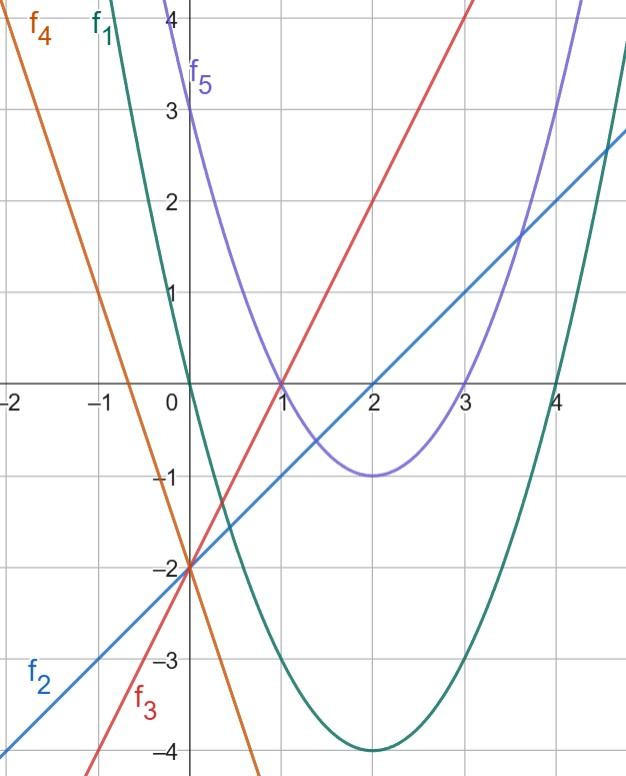
\includegraphics[width=\textwidth]{funcions.jpg} 
\end{minipage}

\newpage
    

% EXERCICI 5
\question (1 punt) Troba el punt d'intersecció (punt on es creuen) les gràfiques de les funcions $f(x) = 2x + 1$ i $g(x) = -x + 4$.


% EXERCICI 6
\question (1 punt) Representa gràficament la funció quadràtica $f(x) = x^2 - 6x + 5$. Calcula:
\begin{parts}
    \part L'orientació i les coordenades del vèrtex.
    \part Els punts de tall amb els eixos horitzontal i vertical.
    \part Dibuixa la gràfica.
\end{parts}

\vspace{0.3cm}

% EXERCICI 7
\question (1 punt) Troba l'expressió algebraica de la funció quadràtica $f(x) = ax^2 + bx + c$ que passa pels punts $A(0, 2)$, $B(1, 3)$ i $C(-1, 5)$.

\vspace{0.3cm}

% EXERCICI 8
\question (1 punt) Observa la gràfica de la funció definida a trossos (adjunta) i respon:
\begin{parts}
    \part Indica el domini i el recorregut de la funció.
    \part Quins són els punts de tall amb els eixos?
    \part Determina els intervals de creixement i decreixement.
    \part Indica els màxims i mínims (especifica si són relatius o absoluts).
    \part És una funció contínua? Si no ho és, indica on no ho és.
\end{parts}

% ESPAI PER A LA IMATGE DE GEOGEBRA
\begin{center}
    \fbox{\begin{minipage}{0.8\textwidth} \centering  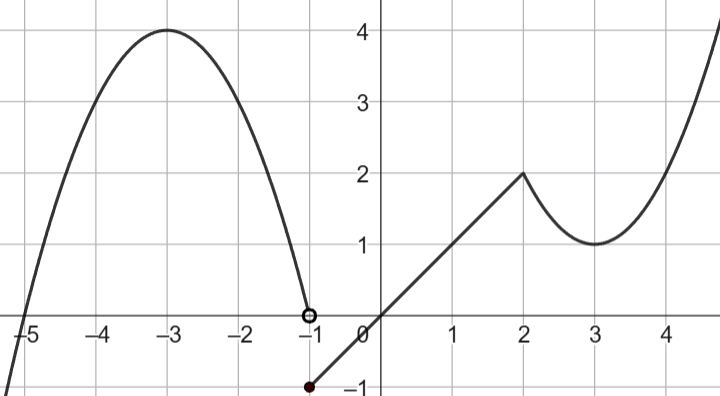
\includegraphics[width=\textwidth]{CaracteristiquesFuncions.png} 
    \end{minipage}}
\end{center}

\vspace{0.3cm}

% EXERCICI 9
\question (1 punt) Unes vambes de col·leccionista valien $120$ € en sortir al mercat (mes 0). Al cap de $3$ mesos, el seu valor és de $170$ €. $3$ mesos després tenen un valor de $225 €$. Suposant un creixement lineal, quin era el valor de les vambes després de 4 mesos i mig? (Extra: representa el problema en un gràfic i comprova si el resultat trobat té sentit)

\newpage
% EXERCICI 10
\question (1 punt) Una empresa d'impressió de samarretes cobra 20 € de despeses fixes de disseny i 8 € per cada samarreta impresa.
\begin{parts}
    \part Escriu l'expressió algebraica de la funció cost $f(x)$ segons el nombre de samarretes $x$.
    \part Què signifiquen el pendent i l'ordenada a l'origen en aquest context?
    \part Calcula el cost total de fer 15 samarretes.
    \part Si hem pagat 140 €, quantes samarretes hem comprat?
\end{parts}

\vspace{0.4cm}

\textbf{Espais lliures per representar.} Indica a quin exercici corresponen \\

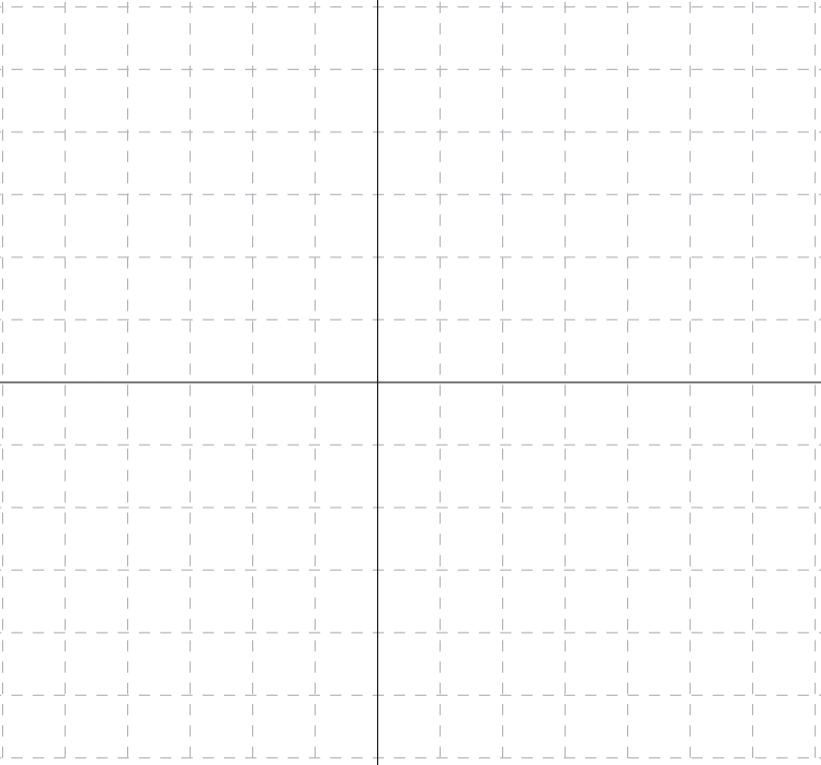
\includegraphics[width=0.5\textwidth]{EixosBuits.png}
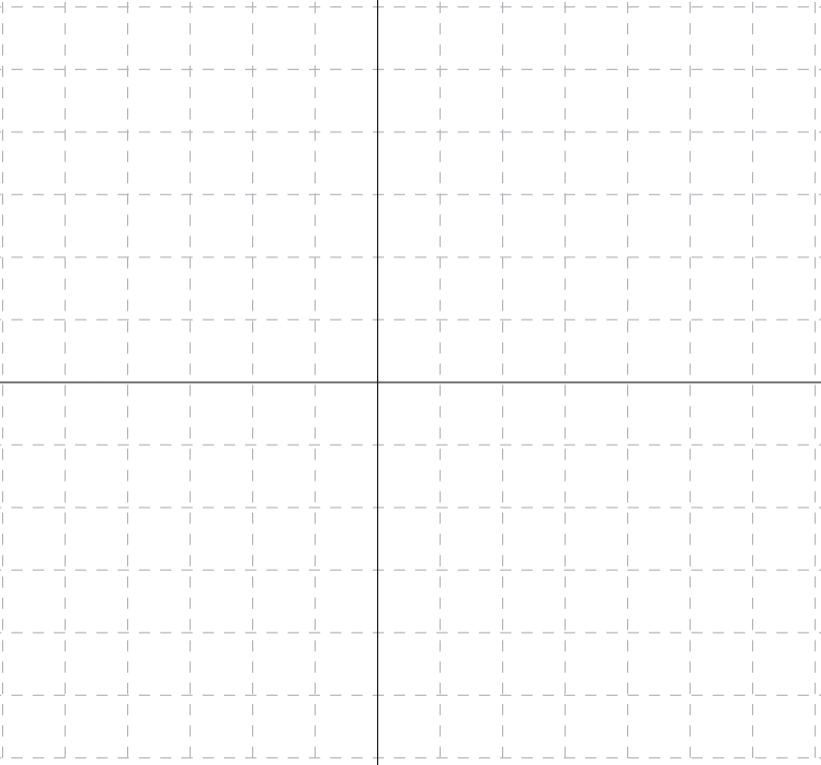
\includegraphics[width=0.5\textwidth]{EixosBuits.png} \\

\vspace{0.4cm}
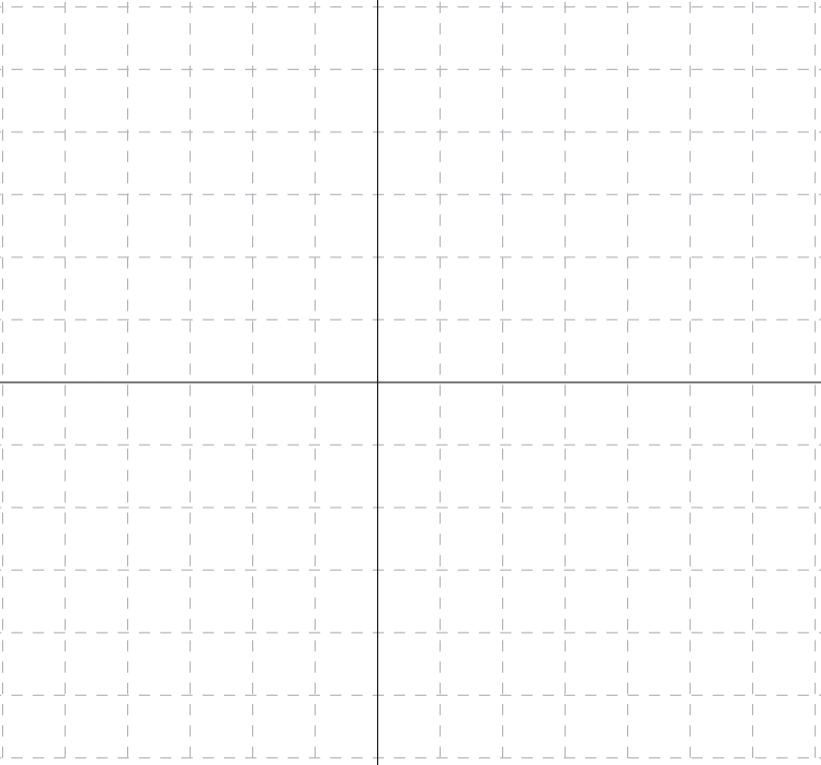
\includegraphics[width=0.5\textwidth]{EixosBuits.png}
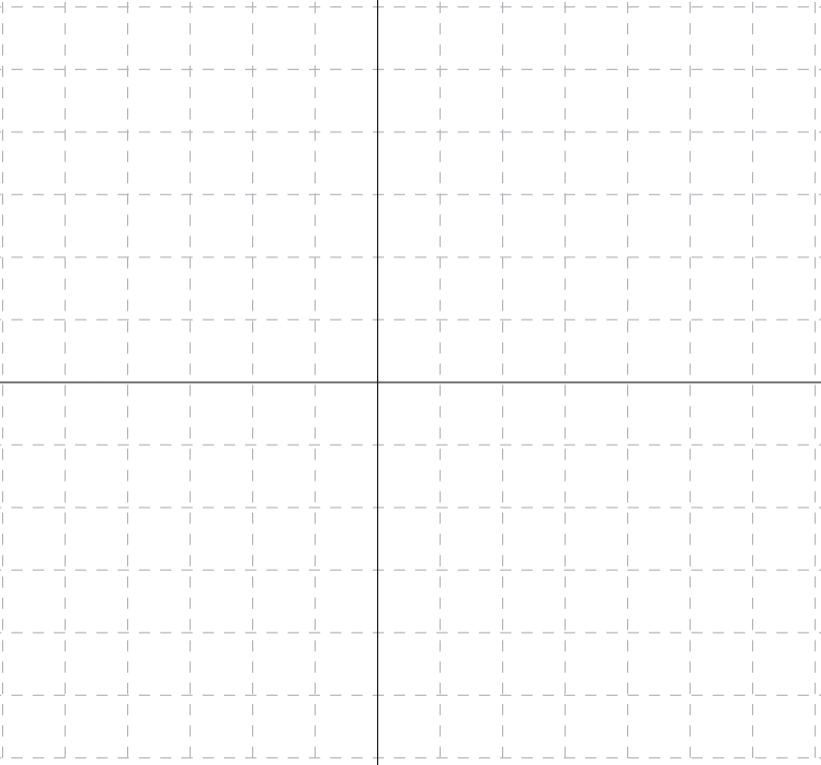
\includegraphics[width=0.5\textwidth]{EixosBuits.png}

\end{questions}
\end{document}